\documentclass[12pt]{report}
\usepackage[a4paper, total={16cm, 24cm}]{geometry}
\usepackage[greek]{babel}	
\usepackage[Glenn]{fncychap}
\usepackage[backend=biber]{biblatex}
\usepackage{listings}
\usepackage{multicol}
\usepackage{xcolor}
\usepackage{caption}
\usepackage{textcomp}
\usepackage{graphicx}
\usepackage{wrapfig}

\addbibresource{thesis.bib}
\graphicspath{{img/}}

\definecolor{codegray}{rgb}{0.5,0.5,0.5}
\definecolor{backcolour}{rgb}{0.95, 0.95, 0.92}

\lstdefinestyle{style}{
    backgroundcolor=\color{backcolour},   
    basicstyle=\ttfamily\footnotesize,
    breakatwhitespace=false,         
    breaklines=true,                 
    keepspaces=true,                 
    showspaces=false,                
    showstringspaces=false,
    showtabs=false,                  
    tabsize=2
}
\lstset{style=style}

\author{Βεϊσάκης Μανούσος}
\title{Μοντελοποίηση συστημάτων αποθήκευσης, με σκοπό την αυξημένη διείσδυση των ΑΠΕ στο δίκτυο ηλεκτρικής ενέργειας}
\date{\today}

\begin{document}
\maketitle
\tableofcontents
\chapter*{{\latintext{Abstract}}}
Η μεταστροφή σε φιλικότερες για το περιβάλλον πηγές ενέργειας είναι αναπόφευκτη, καθώς η ανάγκη για ένα οικολογικότερο μέλλον, αλλά και η επιβάρυνση των χωρών με τέλη εκπομπών, καθιστούν τις συμβατικές μονάδες παραγωγής ενέργειας,
ασύμφορες. Η μεγαλύτερη διείσδυση των ΑΠΕ, όμως, στο δίκτυο ηλεκτρικής ενέργειας προϋποθέτει την ύπαρξη αποθηκευτικών μέσων, που θα δεσμεύουν την παραπανήσια ενέργεια που παράγουν οι ΑΠΕ κατά τις ώρες
χαμηλής ζήτησης και θα την διαθέτουν στους καταναλωτές, κατά τις ώρες υψηλότερης ζήτησης. 
Αυτό συμβαίνει διότι η παραγωγή των ΑΠΕ εξαρτάται από τις καιρικές συνθήκες, κανοντάς την απρόβλεπτη. Συνεπώς ένα δίκτυο ηλεκτρικής ενέργειας δεν να βασίζεται εξ ολοκλήρου σε αυτές.

Σε πολλά μέρη μάλιστα η εγκατάσταση ΑΠΕ πάνω από ένα όριο απαγορεύεται, διότι υπερβαίνεται το όριο ισχύς του δικτύου, αλλά κυρίως διότι είναι ανούσιο. Χωρίς κάποιον τρόπο να διαμοιράζεται η ενέργεια κατά τις ώρες μεγάλου φόρτου, 
η παραγώμενη ενέργεια απλά δεν είναι αξιοποιήσιμη.
Με την αναμενώμενη εξέλιξη του δικτύου σε {\latintext{smart-grid}} και την ένταξη των {\latintext{micro-grid}} στην κοινωνία, προβλέπεται να υπάρξουν σημαντικές αλλαγές στον τρόπο που χειριζόμαστε την ενέργεια. Τα έξυπνα
δίκτυα εκπροσωπούν μία αμφίδρομη σχέση μεταξύ της παραγωγής και της κατανάλωσης, καθώς ο ίδιος ο πολίτης στην σημερινή εποχή, μέσω των ΑΠΕ, μπορεί να είναι παραγωγός. Για τους παραπάνω λόγους η συζητήσεις 
περί ένταξης μεγάλων σταθμών αποθήκευσης ενέργειας στο δίκτυο, έχουν ενταθεί. 

Στην παρούσα εργασία αναπτύχθηκε ένα πρόγραμμα σε γλώσσα {\latintext{Python}}, το οποίο υπολογίζει το μέγεθος του αποθηκευτικού συστήματος που χρειάζεται μια περιοχή, έτσι ώστε να αυξηθούν οι ΑΠΕ στο δίκτυό της. 
Στα αποτελέσματα του προγράμματος περιλαμβάνονται το κόστος του τελικού συστήματος, καθώς και το πώς θα μεταβληθεί η καμπύλη του φορτίου του δικτύου, μέσω αυτής της προσαρμογής.
\chapter*{Εισαγωγή}
Τον 20ο αιώνα έγινε αντιληπτό ότι ο νέος τρόπος παραγωγής που έφερε η βιομηχανική επανάσταση δεν ήταν βιώσιμος. Πρώτη φορά η ανθρωπότητα είχε την ικανότητα
να επηρεάσει σε τέτοιο βαθμό το οικοσύστημα της Γης. Ήταν εμφανές πια, ότι έπρεπε να βρεθεί ένας πιο οικολογικός τρόπος για να καλυφθούν οι όλο και αυξανόμενες ανάγκες των ανθρώπων, εάν 
ήθελε η ανθρωπότητα να αφήσει έναν, αν όχι καλύτερο, ίδιου επιπέδου κόσμο, στις επόμενες γενιές.
Έτσι πολλές χώρες αποφάσισαν να καθιερώσουν νομοθεσίες, οι οποίες θα επιβάλλουν όλο και χαμηλότερη
εκπομπή ρύπων διοξειδίου του άνθρακα, προωθώντας μία μεταστροφή σε καθαρότερες πηγές ενέργειας, σε αντίθεση με τις συμβατικές μονάδες παραγωγής ηλεκτρικής ενέργειας.
Όλο αυτό παρότρυνε τον επιστημονικό και τεχνολογικό τομέα να ερευνήσει ακόμα περισσότερο τις φιλικότερες για το περιβάλλον ενεργειακές πηγές, τις επονομαζόμενες Ανανεώσιμες Πηγές Ενέργειας (ΑΠΕ). 
Λόγω της εξέλιξης της τεχνολογίας, της εύρεσης φθηνότερων υλικών και της μαζικής παραγωγής, οι βιομηχανίες κατάφεραν να μειώσουν το κόστος των ΑΠΕ και παράλληλα να αυξήσουν την αποδοτικότητά τους.
Έτσι οι ΑΠΕ δεν ήταν πια μία ερευνητική ιδέα, αλλά μία πρωσιτή λύση, που συνυπολογίζοντας τα πρόστιμα στα ορυκτά καύσιμα, ανταγωνίζεται τις συμβατικές.
Από τα παραπάνω συμπεραίνει κανείς, ότι η μεταστροφή στις ΑΠΕ είναι αναπόφευκτη και θα είναι το επίκεντρο των προσοχής για πολλά χρόνια ακόμη, όσον αφορά τον ενεργειακό τομέα. 

Παρ'όλα αυτά οι ΑΠΕ έχουν ένα πολύ σοβαρό μειονέκτημα, αυτό της αβεβαιότητας. Σε αντίθεση με τις συμβατικές πηγές ενέργειας (π.χ. λιγνίτης, φυσικό αέριο κ.α.), οι οποίες
έχουν μία σταθερή παραγωγή, η παραγωγή των ΑΠΕ βασίζεται, εκ φύσεως, στις καιρικές συνθήκες. Αυτό παρουσιάζει πολλές δυσκολίες όσον αφορά την ένταξή τους στο δίκτυο ηλεκτρικής ενέργειας.
Αρχικά δεν μπορεί ένα κράτος να βασιστεί σε αυτές για την πλήρη κάλυψη του φορτίου του, χωρίς να υπάρχει σε ένα βαθμό μία σταθερή πηγή ενέργειας, πάνω στην οποία θα ενταχθούν οι ΑΠΕ.
Για παράδειγμα, τα φωτοβολταϊκά (ΦΒ) παράγουν ισχύ μόνο τις ώρες με συγκεκριμένη ηλιοφάνεια, ενώ το μεγαλύτερο φορτίο στο δίκτυο παρουσιάζεται τις βραδυνές ώρες. Αυτό σημαίνει ότι ενώ μπορεί να υπάρχει επαρκή ισχύς ΑΠΕ
σύμφωνα με τις ανάγκες του δικτύου, αυτή δεν παράγεται τις αναγκαίες ώρες, με συνέπεια όλη αυτή η παραγώμενη ενέργεια, να μην είναι αξιοποιήσιμη. Οι ΑΠΕ δηλαδή εξυπηρετούν μέχρι στιγμής, την κάλυψη του φορτίου αιχμής
ενός δικτύου (ξαφνικές διακυμάνσεις πάνω από το σύνηθες) και η διείσδυσή τους πάνω από ένα βαθμό, έχει περισσότερα κόστη, παρά οφέλη. 

Ο μόνος τρόπος για να είναι εφικτή η άυξηση της διείσδυσης των ΑΠΕ στο δίκτυο και ίσως η εξ ολοκλήρου τροφοδοσία του δικτύου με αυτές, είναι να υπάρχει τρόπος να αποθηκευτεί η παραπανήσια ενέργεια κατά την ώρα παραγωγής της
και η διάθεσή της στο δίκτυο κατά τις ώρες αυξημένης ζήτησης. Ευτυχώς, η αποθηκευτική τεχνολογία έχει αναπτυχθεί σε μεγάλο βαθμό τις τελευταίες δεκαετίες (βλ. Κεφάλαιο \ref{chap:storage}) και δίνεται η δυνατότητα επιλογής
διαφορετικών αποθηκευτικών μέσων, ανάλογα με τις ανάγκες. Κάποια απευθήνονται για παράδειγμα σε βραχυπρόθεσμες αποθηκεύσεις, ενώ άλλα μπορεί να απευθύνονται σε ανάγκες υψηλής ισχύος. 

Η ένταξη των ΑΠΕ και πόσο μάλλον των αποθηκευτικών συστημάτων στο δίκτυο, θα πρέπει να συνοδευτεί με μεταρρυθμίσεις στην ίδια τη λειτουργία του δικτύου. Μέχρι σήμερα, το δίκτυο ηλεκτρικής ενέργειας ακολουθεί 
το συμβατικό σχήμα παραγωγού-καταναλωτή. Όταν είχε πρωτοσχεδιαστεί αυτή η διάταξη δεν είχε υπολογιστεί, ότι και ο ίδιος ο καταναλωτής θα μπορεί να γίνει παραγωγός και να προσφέρει ενέργεια στο δίκτυο.
Στη σημερινή εποχή όμως, η εγκατάσταση ΑΠΕ σε οικιακό επίπεδο είναι κάτι το όλο και πιο σύνηθες, η σχέση μεταξύ παραγωγού και καταναλωτή γίνεται όλο και περισσότερο πιο αμφίδρομη.
Αυτή την ανάγκη έρχονται να εξυπηρετήσουν τα έξυπνα δίκτυα ({\latintext{smart-grids}}). Σε συνδυασμό με τα ηλεκτρικά αυτοκίνητα \footnote{Την στιγμή που γράφεται το κείμενο κατατίθεται νομοσχέδιο προς ψήφιση στην ελληνική Βουλή,
για την απαγόρευση πώλησης αυτοκινήτων εσωτερικής καύσης από το 2035, αλλά και υποχρεωτικής χρήσης αυτοκινήτων μηδενικών εκπομπών για τα ταξί εντός Αττικής και Θεσσαλονίκης από το 2027 \parencite{energypress1105}.}, 
οι μπαταρίες αυτές θα μπορούν να τροφοδοτούν το δίκτυο με επιπρόσθετη ενέργεια σε συνθήκες υψηλής ζήτησης.

\begin{wrapfigure}{r}{0.4\textwidth}
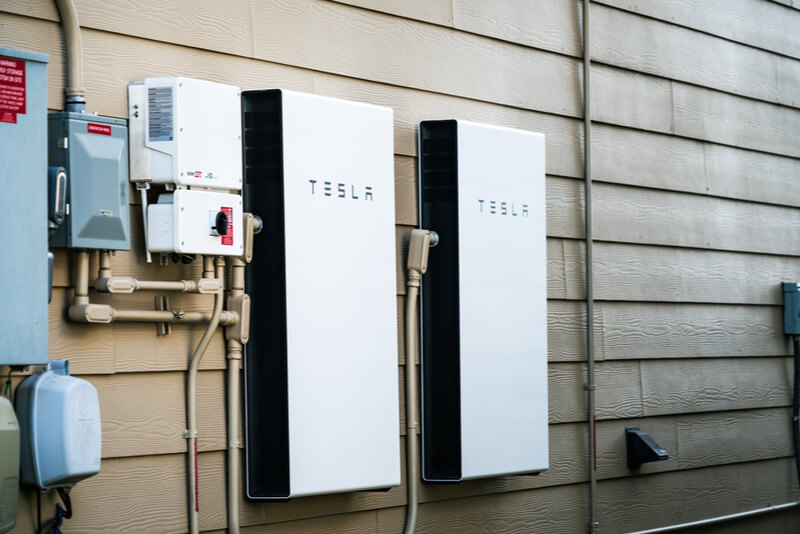
\includegraphics[width=0.4\textwidth]{powerwall}
\captionsetup{name=Εικόνα}
\caption{{\latintext{Tesla Powerwall}}}
\label{fig:powerwall}
\end{wrapfigure}
Αντίστοιχη χρήση έχει αρχίσει και σε πειραματικό επίπεδο στο εξωτερικό με τις οικιακές μπαταρίες (βλ. {\latintext{Tesla Powerwall}} στην Εικόνα \ref{fig:powerwall}). 
Αυτές αρχικά μπορούν να χρησιμοποιηθούν για ασφάλεια σε περιοχές με συχνές διακοπές ρεύματος, με το να αποθηκεύουν
ηλεκτρική ενέργεια από το δίκτυο και να τροφοδοτούν το σπίτι σε περίπτωση διακοπής. Υπάρχει η λειτουργία μάλιστα να προγραμματιστεί η μπαταρία να απορροφάει ενέργεια από το δίκτυο μόνο τις ώρες με φθηνότερο κόστος (π.χ. νυχτερινό
ρεύμα). Η πραγματική αξία όμως αυτών των τεχνολογιών εμφανίζεται όταν συνδυαστούν με ΑΠΕ. Όση παραγωγή ενέργειας δεν αξιοποιείται επιτόπου, αποθηκεύεται στις μπαταρίες, από τις οποίες ο χρήστης αντλεί ενέργεια για τις βραδυνές
τους καταναλώσεις. Με την χρήση των έξυπνων δικτύων που προαναφέρθηκαν, ο παραγωγός και ο καταναλωτής μπορούν να έχουν αμοιβαίο κέρδος.
Το δίκτυο κάνει ανοιχτή πρόσκληση σε όποιον ενδιαφερόμενο, ώστε να μπορεί να του αντλεί ενέργεια από τις μπαταρίες του, συγκεκριμένες περιόδους του χρόνου (π.χ. Ιούλιος-Σεπτέμβριος που υπάρχει η μέγιστη ζήτηση). Κάθε περισταστικό
διαρκεί κάποιες ώρες (συνήθως τις μεσημεριανές), ενώ υπάρχει όριο στα πόσα περιστατικά θα μπορεί να υπάρξουν στον ενδιαφερόμενο μέσα σε αυτήν την περίοδο (π.χ. 50). Στη συνέχεια το δίκτυο είναι υπεύθυνο να πληρώσει το ποσό 
που έχει εγγυηθεί, το οποίο είναι αρκετά ικανοποιητικό. Με αυτό το ποσό όμως κερδίζουν και οι δύο πλευρές. Το κόστος που θα είχε να λειτουργήσει μία παραπάνω μονάδα παραγωγής ηλεκρικής ενέργειας, 
μόνο για αυτά τα συγκεκριμένα περιστατικά μέσα στην περίοδο, είναι κατά πολύ μεγαλύτερο από την "αγορά" της ενέργειας αυτής από τους ίδιους τους καταναλωτές. Από την άλλη ο καταναλωτής μπορεί να ορίσει το ποσό της ενέργειας
που θα επιτρέπει να δίνει η μπαταρία στο δίκτυο και αν συνδυαστεί αυτό με κάποιο διάστημα που αυτός λείπει από το σπίτι, τότε η ενέργεια που παράγεται από τις ΑΠΕ στο σπίτι του δεν θα πηγαίνει χαμένη καθώς
θα μπορεί να πωλείται ενώ λείπει. Με αυτόν τον τρόπο, αν οι κάτοικοι της περιοχής ενταχθούν σε αυτό το πρόγραμμα, φτιάχνεται μία μεγάλη εικονική μπαταρία για να στηρίζει το δίκτυό της.

Με την ίδια λογική και με τη χρήση των {\latintext{micro-grid}} θα μπορούν ολόκληρες περιοχές να τροφοδοτούνται σε μεγάλο βαθμό μεταξύ τους, μειώνοντας και το ρίσκο διακοπής ρεύματος από τυχόν βλάβη στον κεντρικό παραγωγό. 
Οι κάτοικοι με ΑΠΕ, γεννήτριες, μπαταρίες κ.α. θα υποστηρίζουν το δίκτυο της περιοχής τους, με το αντίστοιχο οικονομικό κέρδος από το δίκτυο. Έτσι βγαίνουν όλοι κερδισμένοι, ακολουθώντας την λογική που αναφέρθηκε
στην προηγούμενη παράγραφο.

Όλα αυτά είναι εξελίξεις, στις οποίες τα έξυπνα δίκτυα μπορούν και θα πρέπει να ανταπεξέλθουν. Η ανθρωπότητα περνάει σε μια εποχή που η χρήση της ενέργειας αλλάζει μορφή, γίνεται αμφίδρομη με στόχο την αποδοτικότητα
και την οικολογία.

Στην εργασία αυτή αναλύονται αρχικά διαφορετικοί τρόποι παραγωγής και αποθήκευσης ενέργειας, ενώ στη συνέχεια γίνεται μία αναλυτική περιγραφή του προγράμματος, καθώς και των εργαλειών που χρειάζονται για τη λειτουργία του.
\chapter{Παραγωγή Ενέργειας}
\chapter{Αποθήκευση Ενέργειας}
\label{chap:storage}
Η αποθήκευση ενέργειας δεν είναι μία καινούργια ανησυχία. Ανέκαθεν ο άνθρωπος αναζητούσε τρόπους να δεσμεύσει ενέργεια για μελλοντική χρήση, απλά τώρα υπάρχει η κατάλληλη τεχνολογία. Στο κεφάλαιο αυτό θα αναφερθούν
συνοπτικά οι κύριες τεχνολογίες αποθήκευσης, που απασχολούν τον ενεργειακό τομέα, των οποίων η χρήση δεν είναι απλά επιστημονικά ενδιαφέρουσα, αλλά και οικονομικά συμφέρουσα.
\section{Αντλησιοταμίευση}
Εδώ και πάνω από έναν αιώνα έχουν εφαρμοσθεί έργα που δεσμεύουν παραπανήσια ενέργεια και την διαθέτουν στο δίκτυο κατά τις ώρες υψηλής ζήτησης. Αναφερόμαστε στα έργα αντλησιοταμίευσης. 
Σύμφωνα το υπουργείο ενέργειας των ΗΠΑ \parencite{energygov1801}, η πρώτη γνωστή χρήση των έργων αντλησιοταμίευσης ήταν  στην Ιταλία και την Ελβετία την δεκαετία το 1890. Οι ίδιες οι ΗΠΑ διαθέτουν 43 τέτοιες μονάδες, οι
οποίες είναι υπεύθυνες για το 93\% της ολικής αποθήκευσης ενέργειας του δικτύου τους.
\chapter{Ανάλυση Προγράμματος}
Παρακάτω θα αναλυθούν οι συναρτήσεις που αποτελούν τον κορμό των λειτουργιών του προγράμματος και που βρίσκονται
στο αρχείο {\latintext{processData.py}}. Η επεξήγηση του κυρίως προγράμματος {\latintext{main.py}} θα γίνει μέσω αυτής της διαδικασίας.

Η πρώτη συνάρτηση ονομάζεται {\latintext{formatData}} και σκοπός της είναι να μετατρέψει τα δεδομένα
σε μορφή που θα επιτρέψει και θα διευκολύνει την επεξεργασία τους.

Τα δύο κύρια αρχεία δεδομένων που χρησιμοποιεί το πρόγραμμα είναι η χρονοσειρά του φορτίου του δικτύου και η 
χρονοσειρά της παραγώμενης ισχύος των ΦΒ, για την συγκεκριμένη περιοχή. 

Τα δεδομένα για το φορτίο του δικτύου λαμβάνονται έτοιμα για την περιοχή που θα επιλεχθεί, από το αρχείο στο οποίο
είναι αποθηκευμένα με όνομα {{\latintext{data/}}\textit{<περιοχή>}{\latintext{\_gridload.csv}}. 
Ο χρήστης στην αρχή του προγράμματος ζητείται να διαλέξει μία από τις περιοχές που αναγράφονται και ανάλογα με την
επιλογή του (1-5), επιλέγεται το κατάλληλο αρχείο από τον παραπάνω φάκελο.

{\latintext{
\begin{lstlisting}[language=Python] 
print("\nSelect examination area from the list below (1-5)")
place = int(input("[1] Chania\n[2] Rethymno\n"
                  + "[3] Heraklio\n[4] Ag.Nikolaos\n[5] Moires\n"))

while place > 5 or place < 1:
    print("\nInvalid answer. Please choose one of the below:")
    place = int(input("[1] Chania\n[2] Rethymno\n"
                      + "[3] Heraklio\n[4] Ag.Nikolaos\n[5] Moires\n"))

\end{lstlisting}
}}

Όσον αφορά τα δεδομένα για την παραγώμενη ισχύς από τα ΦΒ, αυτά κατεβαίνουν από την ιστοσελίδα του 
{\latintext{PV-GIS}} μέσω του {\latintext{API}} του. Το αίτημα για τα δεδομένα γίνεται 
μέσω της εντολής {\latintext{curl}} και τα δεδομένα αυτά αποθηκεύονται με τη σειρά τους στο αρχείο {\latintext{data/pv\_production.csv}}.
Για να γίνει το αίτημα αυτό στην ιστοσελίδα, θα πρέπει να δωθούν κάποιες παράμετροι, μέσα στις οποίες είναι και οι 
συντεταγμένες της περιοχής. Συνεπώς ανάλογα με την επιλογή του χρήστη, οι συντεταγμένες αποθηκεύονται σε δύο 
μεταβλητές, {\latintext{lat}} και {\latintext{lon}}. Αυτές αντλούνται από ένα {\latintext{dictionary}}, το οποίο
ορίζεται στην αρχή του προγράμματος για να είναι εφικτή η εύκολη τροποποίησή του ανάλογα με τις ανάγκες του χρήστη.
Για τον ίδιο λόγο ορίζονται στην αρχή του προγράμματος και οι υπόλοιπες μεταβλητές που χρειάζεται η ιστοσελίδα, 
αλλά και όλο το πρόγραμμα.

{\latintext{
\begin{lstlisting}[language=Python] 
places = {
    1: (35.512, 24.012),
    2: (35.364, 24.471),
    3: (35.343, 25.153),
    4: (35.185, 25.706),
    5: (35.050, 24.877)
}
\end{lstlisting}
}}

{\latintext{
\begin{lstlisting}[language=Python] 
lat = str(places[place][0])
lon = str(places[place][1])
\end{lstlisting}
}}

Η συνάρτηση {\latintext{formatData}} δέχεται ως ορίσματα τις δύο χρονοσειρές και τις μετατρέπει σε έναν πίνακα που η κάθε του σειρά
είναι μία μέρα του χρόνου και κάθε στήλη του είναι η αντίστοιχη ώρα της ημέρας, κατά την οποία πάρθηκε η μέτρηση. 
Στο τέλος, η συνάρτηση επιστρέφει δύο πίνακες οι οποίοι έχουν 365 γραμμές και 24 στήλες.

Για την μοντελοποίηση του συστήματος αποθήκευσης θα χρειαστεί να δημιουργηθεί ένα αντικείμενο μπαταρίας, το οποίο θα 
μπορεί να φορτίζει και να ξεφορτίζει, να περιέχει όλα τα λειτουργικά χαρακτηριστικά της μπαταρίας και να μπορεί να αυξάνεται
η χωρητικότητά της, με το να προστίθεται σε αυτήν και άλλες ίδιες μπαταρίες, σαν να υπήρχε ένα σύμπλεγμα μπαταριών.
Στην αρχή του προγράμματος δίνεται η δυνατότητα στον χρήστη να επιλέξει το είδος της μπαταρίας, από την οποία θα αποτελείται το σύστημα.

{\latintext{
\begin{lstlisting}[language=Python] 
print("\nChoose battery type:")
type = int(input("[1] Lead-Carbon (300,000.00/MWh)\n"
                 + "[2] Lithium-Ion (500,000.00/MWh)\n"))

while type > 2 or type < 1:
    print("\nInvalid answer. Please choose one of the below:")
    type = int(input("[1] Lead-Carbon\n"
                     + "[2] Lithium-Ion\n"))

if type == 1:
    bat_type = path + "/thesis/data/lead_carbon.json"
else:
    bat_type = path + "/thesis/data/lithium_ion.json"
\end{lstlisting}
}}

Η επιλογή του χρήστη μετατρέπεται σε όνομα αρχείου {\latintext{json}}. Με βάση αυτό το αρχείο δημιουργείται η αρχική αναπάρασταση
μίας μπαταρίας. Αν το αρχείο δεν βρίσκεται στην σωστή μορφή ή δεν υπάρχει καθόλου, το πρόγραμμα τερματίζει με το να ενημερώνει για το
είδος του σφάλματος.

{\latintext{
\begin{lstlisting}[language=Python] 
try:
    bat = Battery.from_json(bat_type)
except Exception as err:
    print("\nFailed to instantiate battery object from json file...\n")
    sys.exit(err)
\end{lstlisting}
}}

Οι υπολογισμοί που ακολουθούν απο εδώ και πέρα, εφαρμόζονται για κάθε σειρά των πινάκων φορτίου δικτύου και παραγωγής ΦΒ,
δηλαδή για κάθε ημέρα του χρόνου. Στη συνέχεια αυξάνονται οι μπαταρίες κατά μία και ξανατρέχει το πρόγραμμα από την αρχή.
Ουσιαστικά υπάρχουν δύο βρόγχοι {\latintext{for}} ο ένας μέσα στον άλλο.
Το πρόγραμμα τερματίζει όταν ένα από τα παρακάτω σενάρια επιτευχθεί.

\begin{enumerate}
\item Όταν όλη η παραγόμενη ενέργεια από τις ΑΠΕ, αξιοποιείται.
\item Όταν οι ΑΠΕ μαζί με τις μπαταρίες τροφοδοτούν το 100\% του δίκτυου.
\item Όταν το κόστος του συστήματος αποθήκευσης, φτάσει το μέγιστο αποδεκτό από τον χρήστη.
\end{enumerate}

Για να επιτευχθεί η τρίτη συνθήκη, δίνεται η δυνατότητα στον χρήστη να εισάγει ένα μέγιστο κόστος που μπορεί να διαθέσει. 
O χρήστης μπορεί να εισάγει τον αριθμό 0, αν δεν θέλει να υπάρχει κάποιος οικονομικός περιορισμός.

Μετά την {\latintext{formatData}} εκτελείται η συνάρτηση {\latintext{wastedEnergy}}. Αυτή δέχεται για ορίσματα δύο σειρές αριθμών,
στην περίπτωσή μας τις μετρήσεις μίας ημέρας για το φορτίο του δικτύου και της παραγώμενης ισχύς των ΦΒ και στη συνέχεια υπολογίζει 
πόση ενέργεια από τα ΦΒ δεν αξιοποιείται μέσα στην ημέρα. Στο τέλος ελέγχει αν η μπαταρία έχει χώρο να αποθηκεύσει αυτήν την ενέργεια και
αν μπορεί, το κάνει. 
\chapter{Τεχνικά Ζητήματα}
Το πρόγραμμα έχει σχεδιασθεί να τρέχει σε περιβάλλον {\latintext{Linux}} και χρησιμοποιεί {\latintext{Python 3}} με τις παρακάτω βιβλιοθήκες:
\begin{multicols}{4}
\begin{itemize}
\item {\latintext{os}}
\item {\latintext{math}}
\item {\latintext{json}}
\item {\latintext{sys}}
\item {\latintext{requests}}
\item {\latintext{numpy}}
\item {\latintext{pandas}}
\item {\latintext{matplotlib}}
\end{itemize}
\end{multicols}
Πέρα από αυτές τις βιβλιοθήκες, το πρόγραμμα χρειάζεται κάποιες εντολές του {\latintext{Linux}} για να λειτουργήσει, οι οποίες είναι:
\begin{multicols}{2}
\begin{itemize}
\item {\latintext{curl}}
\item {\latintext{figlet}}
\end{itemize}
\end{multicols}
Για την γρήγορη και εύκολη σύνθεση του περιβάλλοντος, υπάρχει ένα {\latintext{script}} το οποίο εγκαταστεί όλα τα προαπαιτούμενα σε ένα περιβάλλον {\latintext{Linux}}, το οποίο πρέπει όμως να βασίζεται 
στη διανομή {{\latintext{Debian}}. Σε περίπτωση που δεν χρησιμοποιείται τέτοιου είδους διανομή, ο χρήστης θα πρέπει να εγκαταστήσει χειροκίνητα τις βιβλιοθήκες και τα προγράμματα αυτά. 
Επιπλέον το σύστημα πρέπει να έχει γραφικό περιβάλλον, αλλιώς δεν μπορούν να εμφανιστούν τα διαγράμματα, που δημιουργούνται μέσω της βιβλιοθήκης {\latintext{matplot}}.
Σε αντίθετη περίπτωση, ο χρήστης θα πρέπει να τροποποιήσει τον κώδικα στον τομέα που φτιάχνονται τα διαγράμματα, με σκοπό αντί να εμφανίζονται, το πρόγραμμα να τα αποθηκεύει σε αρχείο εικόνας, το οποία μπορούν
να ανοιχτούν χωρίς γραφικό περιβάλλον.

\chapter{Συμπεράσματα}
\printbibliography
\end{document}

